\documentclass[reqno,a4paper,12pt]{amsart}

\usepackage{amsmath,amssymb,amsthm,geometry,xcolor,soul,graphicx}
\DeclareMathOperator{\sech}{sech}
\usepackage{mathrsfs} %\mathscr{}
%\usepackage{array}
\usepackage{float} % 在tcolorbox中添加table (由于tcolorbox已经是一个box,因此不能直接加table)
\usepackage{subfig} % 多张图放一起
\usepackage{titlesec}
%\usepackage{enumitem}
\usepackage{enumerate}
\usepackage{lipsum}
\usepackage{listings}
\allowdisplaybreaks[4] %align公式跨页
\RequirePackage[most]{tcolorbox}
\usepackage{braket}
%\usepackage{esint} %$\varoiint$ (带圈的二重积分)
%\usepackage[colorlinks,linkcolor=red]{hyperref} %\url{}超链接
\usepackage[scheme=plain,linespread=1,punct=CCT]{ctex}% Chinese support, single line space, narrow-version SBC case punctuations
\setCJKfamilyfont{zhsong}[AutoFakeBold={2.17}]{SimSong-Regular}
\renewcommand{\songti}{\CJKfamily{zhsong}}
%\usepackage{xeCJK}
%\setCJKmainfont{Kai}
\geometry{left=0.7in, right=0.7in, top=1in, bottom=1in}

\renewcommand{\baselinestretch}{1.3}

\title{固体物理第十四次作业}
\author{董建宇 ~~ 2019511017}

\begin{document}

\maketitle

\begin{enumerate}[1.]

\item \textbf{(22.1) $\ddagger$ Weiss Mean Field Theory of a Feeromagnet} \\
Consider the spin-1/2 ferromagnetic Heisenberg Hamiltonian on the cubic lattice: 
\[
	\mathscr{H} = -\frac{J}{2}\sum_{\langle i,j \rangle} \mathbf{S_i\cdot S_j} + g\mu_B\mathbf{B} \cdot \sum_{i} \mathbf{S_i}
\]
Here, $J>0$, with the sum indicated with $\langle i,j \rangle$ means summing over $i$ and $j$ being neighboring sites of the cubic lattices, and $\mathbf{B}$ is the externally applied magnetic field, which we will assume is in the $\hat{z}$ direction for simplicity. The factor of $1/2$ out front is included so that each pair of spins is counted only once. Each site $i$ is assumed to have a spin $\mathbf{S_i}$ of spin $S = 1/2$. Here $\mu_B$ is the conventional Bohr magneton defined to be positive. The fact that the final term has a $+$ sign out front is from the fact that the electron charge is negative, therefore the magnetic moment opposes the spin direction. If one were to assume that these were nuclear spins the sign would be reversed (and the magnitude would be much smaller due to the larger nuclear mass). \\
(a) Focus your attention on one particular spin $\mathbf{S_i}$, and write down an effective Hamiltonian for this spin, treating all other variables $\mathbf{S_j}$ with $j \neq i$ as expectations $\langle \mathbf{S_j} \rangle$ rather than operators. \\
(b) Calculate $\langle \mathbf{S_i} \rangle$ in terms of the temperature and fixed variables $\langle \mathbf{S_j} \rangle$ to obtain a mean-field self-consistency equation. Write the magnetization $M = \vert \mathbf{M} \vert$ in terms of $\langle \mathbf{S} \rangle$ and the density of spins. \\
(c) At high temperature, find the susceptibility $\chi = dM/dH = \mu_0dM/dB$ in this approximation. \\
(d) Find the critical temperature in this approximation. \\ 
$\triangleright$ Write the susceptibility in terms of this critical temperature. \\
(e) Show graphically that in zero external field $(\mathbf{B} = 0)$, below the critical temperature, there are solutions of the self-consistency equation with $M \neq 0$. \\
(f) Repeat parts (a)-(d) but now assuming there is an $S=1$ spin on each site (meaning that $S_z$ takes the values $-1,0,+1$).
\begin{tcolorbox}[breakable, colframe = black, colback = black!5!white]
\begin{enumerate}[(a)]

\item 考虑一个自旋$\mathbf{S_i}$,假设近邻自旋数目为$z$,利用平均场近似,则有效Hamiltonian可以写为:
\[
	H_{eff} = -Jz\mathbf{S_i} \cdot \langle \mathbf{S_j} \rangle + g\mu_B \mathbf{B} \cdot \mathbf{S_i}.
\]

\item 假设磁感应强度方向为$+\hat{z}$方向,则平均自旋方向应指向$-\hat{z}$方向使得能量更低。同时,由于$\mathbf{S_i} = \pm \frac{1}{2}$,能量的可能取值为:
\[
	E = \pm \frac{1}{2}\left( g\mu_BB_z - Jz\langle S_z \rangle \right).
\]
配分函数为:
\[
	Z = e^{\beta(g\mu_BB_z - Jz\langle S_z \rangle)/2} + e^{-\beta(g\mu_BB_z - Jz\langle S_z \rangle)/2}.
\]
则单个自旋磁矩满足方程为:
\[
	m = kT \frac{\partial \ln Z}{\partial B_z} = \frac{g\mu_B}{2} \tanh(\beta(g\mu_BB_z - Jz\langle S_z \rangle)/2).
\]
由于磁矩与自旋关系为$m = -g\mu_B\langle S_z \rangle$,则有:
\[
	\langle S_z \rangle = -\frac{1}{2} \tanh(\beta(g\mu_BB - Jz \langle S_z \rangle)/2).
\]
单位体积的磁矩为:
\[
	M = m\rho V = -g\mu_B \langle S_z \rangle \rho V.
\]
其中$\rho$为自旋数密度。

\item 对于高温环境,$\beta\to0$,则平均自旋满足的方程为:
\[
	\langle S_z \rangle = -\frac{\beta}{4}(g\mu_BB - Jz \langle S_z \rangle).
\]
可以解得:
\[
	\langle S_z \rangle = -\frac{\beta g\mu_BB_z}{4-\beta Jz}.
\]
则可以计算磁化率为:
\[
	\chi = \mu_0 \lim_{B \to 0} \frac{dM}{dB} = \frac{\mu_0 (g\mu_B)^2 \rho V}{4k_BT - Jz} = \frac{\mu_0 (g\mu_B)^2 N}{4k_BT - Jz}
\]
其中$N = \rho V$为体系自旋数目。

\item 其中,磁化率可以写为:
\[
	\chi = \frac{\mu_0(g\mu_B)^2N/4}{k_B(T-T_C)}.
\]
则临界温度为:
\[
	T_C = \frac{Jz}{4k_B}.
\]

\item 选取教材图片如下:可以注意到,两条曲线分别为
\[
	y = \langle \sigma \rangle; ~ y = \frac{1}{2}\tanh(\beta Jz\langle\sigma\rangle/2).
\]
当温度小于临界温度$T_C$时,两条曲线存在$\langle \sigma \rangle \neq 0$的交点,也就意味着体系的磁化强度可以不为0。但是随着温度升高至临界温度以上,两条曲线只存在$\langle \sigma \rangle = 0$唯一一个交点,即外磁场为0时体系的磁化强度为0.
\begin{figure}[H]
	\centering
	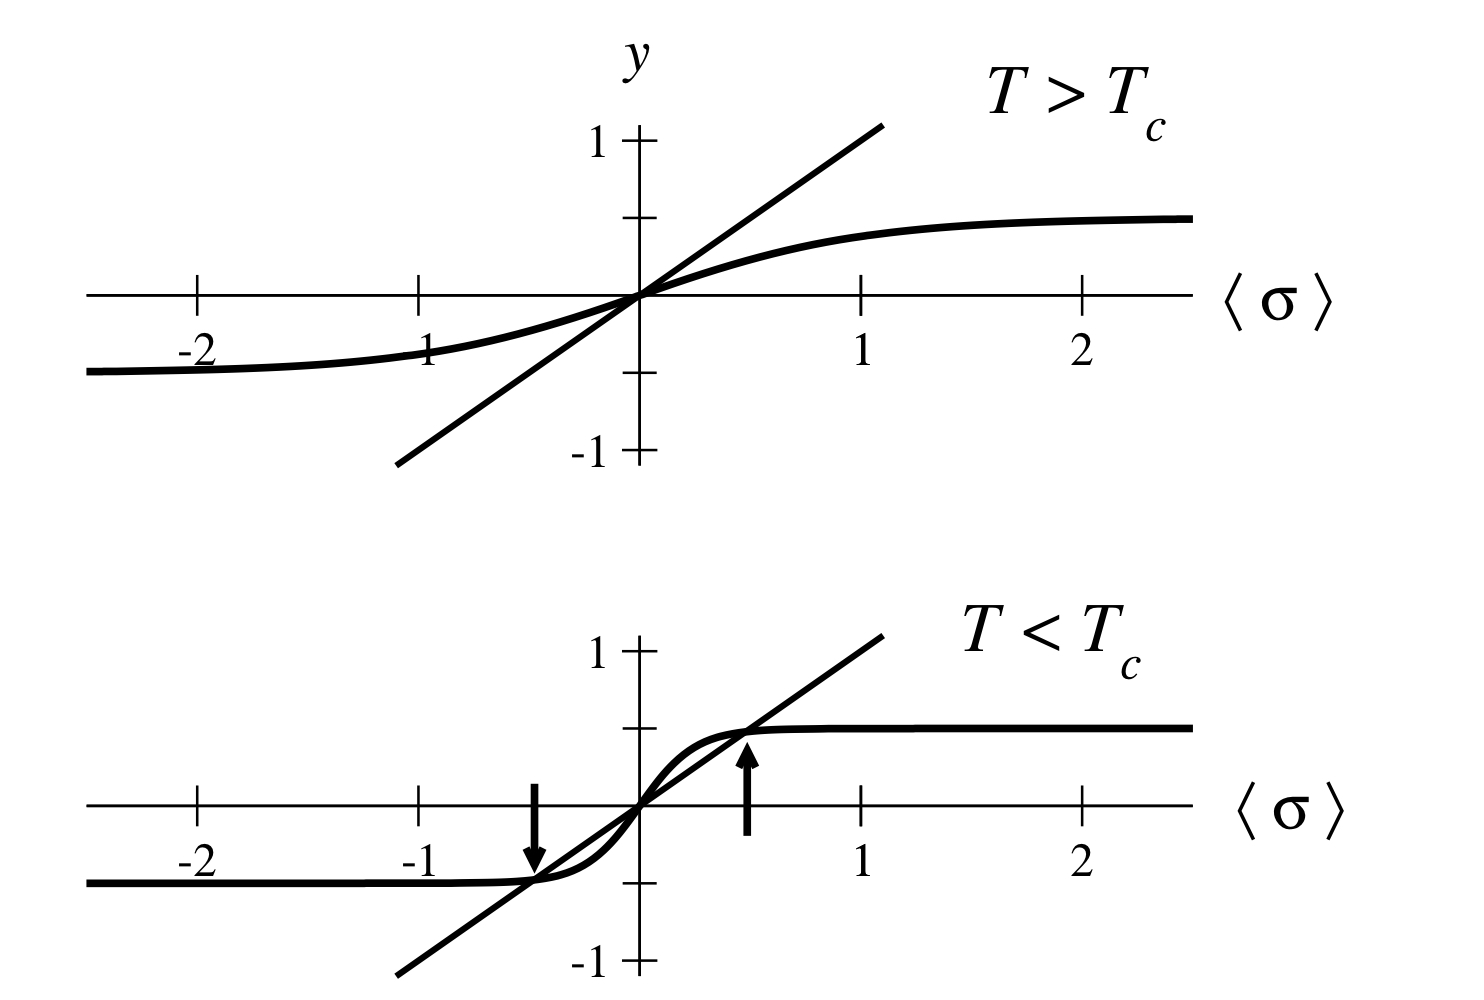
\includegraphics[width = 120mm]{22.1.jpeg}
	\caption{\text{临界温度两侧平均自旋方程两侧函数随自旋变化曲线}}
\end{figure}

\item 当$S=1$,对一个特定的自旋其有效哈密顿量仍为
\[
	\mathcal{H}=\mathbf{S}_i\cdot\left[-J\sum_j\langle\mathbf{S}_j\rangle+g\mu_B\mathbf{B}\right]=\mathbf{S}_i\cdot g\mu_B\mathbf{B}_{i,eff},
\]
其中自旋$\mathbf{S}_i$感受到的有效磁场为
\[
	g\mu_BB_{i,eff}=g\mu_B\mathbf{B}-J\sum_j\langle\mathbf{S}_j\rangle.
\]
体系的配分函数为
\[
	Z=\sum_{S=-1,0,+1}\exp(\beta E)=\exp(\beta g\mu_BB_{eff})+1+\exp(-\beta g\mu_BB_{eff}).
\]
平均自旋为
\[
	\langle S\rangle=\frac{-\exp(\beta g\mu_BB_{eff})+\exp(-\beta g\mu_BB_{eff})}{\exp(\beta g\mu_BB_{eff})+1+\exp(-\beta g\mu_BB_{eff})}=-\frac{2\sinh(\beta g\mu_BB_{eff})}{2\cosh(\beta g\mu_BB_{eff})+1}.
\]
自洽方程为
\[
	\langle S\rangle=-\frac{2\sinh[\beta(g\mu_BB-Jz\langle S\rangle]}{2\cosh[\beta(g\mu_BB-Jz\langle S\rangle)]+1}.
\]
在高温下,自洽方程可以近似为
\begin{gather*}
	\langle S\rangle=-\frac{2}{3}\beta(g\mu_BB-Jz\langle S\rangle),\\
	\Longrightarrow\langle S\rangle=\frac{-\frac{2}{3}\beta g\mu_BB}{1-\frac{2}{3}\beta Jz}.
\end{gather*}
体系的磁极化率为
\[
	\chi=\mu_0\left.\frac{dM}{dB}\right\rvert_{B=0}=\mu_0\left.\frac{d(-Ng\mu_B\langle S\rangle)}{dB}\right\rvert_{B=0}=\frac{\frac{2}{3}\mu_0(g\mu_B)^2N}{k_BT-\frac{2}{3}Jz}=\frac{\frac{2}{3}\mu_0(g\mu_B)^2N}{k_B(T-T_c)},
\]
其中临界温度
\[
	T_c=\frac{2Jz}{3k_B}.
\]

\end{enumerate}
\end{tcolorbox}

\item \textbf{(22.4) Low-Temperature Mean Field Theory} \\
Consider the $S=1/2$ ferromagnet mean field calculation from Exercise 22.1. At zero temperature, the magnet is fully polarized. \\
(a) Calculate the magnetization in the very low temperature limit. Show that the deviation from fully polarized becomes exponentially small as $T$ goes to zero. \\
$\text{(b)}^*$ Now consider a spin $S$ ferromagnet. Determine the magnetization in the low $T$ limit. You can express your result conveniently in terms of the result of Exercise 22.3.
\begin{tcolorbox}[breakable, colframe = black, colback = black!5!white]
\begin{enumerate}[(a)]

\item 由(22.1)可得,在无外加磁场环境下:
\[
	\langle S_z \rangle = \frac{1}{2} \tanh(\beta Jz\langle S_z \rangle/2).
\]
当温度趋向于0时,有$\beta \to \infty$,则有:
\[
	\langle S_z \rangle = \frac{1}{2} \tanh(\beta Jz\langle S_z \rangle/2) \approx \frac{1}{2} - e^{-\beta Jz\langle S_z \rangle}.
\]
注意到
\[
	\lim_{\beta \to \infty} \langle S_z \rangle = \frac{1}{2}.
\]
则有在低温下:
\[
	\langle S_z \rangle = \frac{1}{2} - e^{-\beta Jz/2}.
\]
即体系与完全极化的偏差为$-e^{-\beta Jz/2}$,随着温度的降低指数形式衰减。

\item 对于自旋为$S$的铁磁体,自洽方程为:
\[
	\langle S \rangle = \frac{\sum\limits_{S_z=-S}^S S_z \exp(-\beta Jz\langle S \rangle S_z)}{\sum\limits_{S_z=-S}^S \exp(-\beta Jz\langle S \rangle S_z)} = \frac{\sum\limits_{m_z=0}^{2S} (S-m_z) \exp(-\beta Jz\langle S \rangle m_z)}{\sum\limits_{m_z=0}^{2S} \exp(-\beta Jz\langle S \rangle m_z)}.
\]
当温度趋向于$0K$时,有$\beta\to\infty$,则有:
\[
	\langle S \rangle \approx (S + (S-1)e^{-\beta Jz\langle S \rangle}) (1 - e^{-\beta Jz\langle S \rangle}) \approx S - e^{-\beta Jz\langle S \rangle}.
\]
注意到当$\beta = \infty$时,$\langle S \rangle = S$。则有:
\[
	\langle S \rangle = S - e^{-\beta JzS}.
\]

\end{enumerate}
\end{tcolorbox}

\item \textbf{(22.5) Mean Field Theory for the Antiferromagnet} \\
For this Exercise we use the molecular field (Weiss mean field) approximation for the spin-1/2 $antiferromagnetic$ model on a three-dimensional cubic lattice. The full Hamiltonian is exactly that of Eq. 22.7, except that now we have $J<0$, so neighboring spins want to point in opposite directions (compared to a ferromagnet where $J>0$ and neighboring spins want to point in the same direction). For simplicity let us assume that the external field points in the $\hat{z}$ direction. \\
At mean field level, the ordered ground state of this Hamiltonian will have alternating spins pointing up and down respectively. Let us call the sub-lattices of alternating sites, of alternating sites, sub-lattice $A$ and sub-lattice $B$ respectively (i.e, $A$ sites have lattice coordinates (i,j,k) with $i+j+k$ odd whereas $B$ sites have lattice coordinates with $i+j+k$ even). \\
In mean field theory the interaction between neighboring spins is replaced by an interaction with an average spin. Let $s_A = \langle S^z \rangle_A$ be the average value of the spins on sub-lattice $A$, and $s_B = \langle S^z \rangle_B$ be the average value of the spins on sub-lattice $B$ (we assume that these are also oriented in the $\pm \hat{z}$ direction). \\
(a) Write the mean field Hamiltonian for a single site on sub-lattice $A$ and the mean field Hamiltonian for a single site on sub-lattice $B$. \\
(b) Derive the mean-field self-consistency equations 
\begin{align*}
	&s_A = \frac{1}{2} \tanh(\beta[JZs_B - g\mu_BB]/2) \\
	&s_B = \frac{1}{2} \tanh(\beta[JZs_A - g\mu_BB]/2) 
\end{align*}
with $\beta = 1/(k_BT)$. Recall that $J<0$. \\
(c) Let $B = 0$. Reduce the two self-consistency equations to a single self-consistency equation. (Hint: Use symmetry to simplify! Try plotting $s_A$ versus $s_B$.) \\
(d) Assume $s_{A,B}$ are small near the critical point and expand the self-consistency equations. Derive the critical temperature $T_c$ below which the system is antiferromagnetic (i.e., $s_{A,B}$ become non-zero).  \\
(e) How does one detect antiferromagnetism experimentally? \\
(f) In this mean-field approximation, the magnetic susceptibility can be written as 
\[
	\chi = -(N/2) g\mu_0\mu_B \lim_{B\to 0} \frac{\partial (s_A + s_B)}{\partial B}
\]
(why the factor of $1/2$ out front?). \\
$\triangleright$ Derive this susceptibility for $T>T_c$ and write it in terms of $T_c$. \\
$\triangleright$ Compare your result with the analogous result for a ferromagnet (Exercise 22.1). In fact, it was this type of measurement that first suggested the existence of anti-ferromagnets! \\
$\text{(g)}^*$ For $T<T_c$ show that 
\[
	\chi = \frac{(N/4)\mu_0 (g\mu_B)^2(1-(2s)^2)}{k_BT + k_BT_c(1-(2s)^2)}
\]
with $s$ the staggered moment (ie, $s(T) = \vert s_A(T) \vert = \vert s_B(T) \vert$). \\
$\triangleright$ Compare this low $T$ result with that of part f. \\
$\triangleright$ Give a sketch of the susceptibility at all $T$.
\begin{tcolorbox}[breakable, colframe = black, colback = black!5!white]
\begin{enumerate}[(a)]

\item 考虑位于子晶格$A$上的一个自旋的Hamiltonian为:
\[
	\mathscr{H}_A = -Jz \langle \mathbf{S_B} \rangle \cdot \mathbf{S_A} + g\mu_B\mathbf{B} \cdot \mathbf{S_A}.
\]
同理可得,位于子晶格$B$上的一个自旋的Hamiltonian为:
\[
	\mathscr{H}_B = -Jz \langle \mathbf{S_A} \rangle \cdot \mathbf{S_B} + g\mu_B\mathbf{B} \cdot \mathbf{S_B}.
\]

\item 根据题目假设,有:
\[
	\langle S_A \rangle = s_A, ~ \langle S_B \rangle = s_B.
\]
考虑位于子晶格$A$上的一个自旋,配分函数可以写为:
\[
	Z = e^{\beta(Jzs_A - g\mu_BB)/2} + e^{-\beta(Jzs_A - g\mu_BB)/2}.
\]
自由能为$F = -k_BT\ln Z$,则可以计算平均自旋为:
\[
	s_A = \frac{1}{g\mu_B} \frac{\partial F}{\partial B} = \frac{1}{2} \tanh(\beta(Jzs_B - g\mu_BB)/2).
\]
同理可知,对于$s_B$的自洽方程为:
\[
	s_B = \frac{1}{2}\tanh(\beta(Jzs_B - g\mu_BB)/2).
\]

\item 当外磁场的磁感应强度为$B = 0$时,自洽方程为:
\begin{align*}
	&s_A = \frac{1}{2} \tanh(\beta Jzs_B/2); \\
	&s_B = \frac{1}{2} \tanh(\beta Jzs_A/2).
\end{align*}
容易观察得知:上述两个方程有较好的对称性,满足$y = f(x)$,同时还有$x = f(y)$,则有:$f(x) = \pm x$。注意到由于体系为反铁磁序,则有$s_A \neq s_B$,则有:$s_A = -s_B$。所以上述自洽方程的解为:
\[
	s_A = -s_B = \frac{1}{2}\tanh(\beta Jzs_B/2) = -\frac{1}{2} \tanh(\beta Jzs_A/2).
\]
则可以将自洽方程组简化为单一自洽方程:
\[
	s = -\frac{1}{2} \tanh(\beta Jzs/2).
\]
其中$s$可以分别为$s_A$或$s_B$。

\item 注意到对于反铁磁序,Hamiltonian中$J<0$,则自洽方程可以写为:
\[
	s = \frac{1}{2} \tanh(\beta \vert J \vert zs/2).
\]
此时,与铁磁序体系对应的自洽方程一致,则可以得到临界温度为:
\[
	T_c = \frac{\vert J \vert z}{4k_B} = -\frac{Jz}{4k_B}.
\]

\item 在实验上,我们可以用对自旋敏感的中子散射探测反铁磁序,对于晶格常数为$a$的简单立方晶格,我们将看到处于$k = 2n\pi/(2a)$的散射峰。此时探测出反铁磁序。但当超过临界温度后由于反铁磁序被破坏,这些衍射峰将消失。

\item 由于子晶格$A$与子晶格$B$分别各含有$N/2$个格点,所以计算磁化率时存在$1/2$因子。 \\
$\triangleright$ 当温度较高时,$\beta \to 0$,则自洽方程组可以写为:
\begin{align*}
	&s_A = \frac{\beta}{4}(Jzs_B - g\mu_BB); \\
	&s_B = \frac{\beta}{4}(Jzs_A - g\mu_BB).
\end{align*}
联立上式可得:
\[
	s_A + s_B = -\frac{2g\mu_BB\beta}{4-\beta Jz}.
\]
则当温度大于临界温度时,磁化率为:
\[
	\chi = -\frac{N}{2}g\mu_0\mu_B \lim_{B\to 0} \frac{\partial (s_A+s_B)}{\partial B} = \frac{N\mu_0\beta(g\mu_B)^2}{4-\beta Jz} = \frac{1}{4} \frac{N\mu_0(g\mu_B)^2}{k_B(T+T_c)}.
\]
$\triangleright$ 对比铁磁序体系,可以注意到铁磁体系高于临界温度的磁化率服从$\frac{1}{T-T_c}$衰减,而反铁磁体系高于临界温度的磁化率服从$\frac{1}{T+T_c}$衰减。根据磁化率随温度变化曲线的渐近线,可以确定体系是铁磁序还是反铁磁序。 

\item \color{blue}{答案思路太妙了} \\
\color{black}
对自洽方程组关于磁感应强度$B$求导,可得:
\begin{align*}
	&\left. \frac{\partial s_A}{\partial B} \right\vert_{B=0} = \left( \left. \frac{\beta Jz}{4}\frac{\partial s_B}{\partial B} \right\vert_{B=0} - \frac{\beta g\mu_B}{4} \right) \sech^2(\beta Jzs_B/2); \\
	&\left. \frac{\partial s_B}{\partial B} \right\vert_{B=0} = \left( \left. \frac{\beta Jz}{4}\frac{\partial s_A}{\partial B} \right\vert_{B=0} - \frac{\beta g\mu_B}{4} \right) \sech^2(\beta Jzs_B/2).
\end{align*}
注意到$s_A = -s_B = s$,则有:
\[
	\sech^2(\beta Jzs_A/2) = \sech^2(\beta Jzs_B/2) = \sech^2(\beta Jzs/2) = 1 - \tanh^2(\beta Jzs/2) = 1-(2s)^2.
\]
自洽方程组对磁感应强度的导数方程组加和,可得:
\[
	\left. \frac{\partial (s_A + s_B)}{\partial B} \right\vert_{B=0} = \left( \frac{\beta Jz}{4}\left. \frac{\partial (s_A + s_B)}{\partial B} \right\vert_{B=0} - \frac{\beta g\mu_B}{2} \right) (1-(2s)^2)
\]
其中,磁化率为$\chi = \left. \frac{\partial (s_A + s_B)}{\partial B} \right\vert_{B=0}$,可得:
\[
	\chi = \frac{(N/4)\mu_0(g\mu_B)^2(1-(2s)^2)}{k_B(T+T_c(1-(2s)^2))}.
\]
当温度$T>T_c$时,$s=0$,则磁化率与$(f)$中结论相同,当温度$T<T_c$时,$(1-(2s)^2)$迅速下降为0,则磁化率也迅速下降为0。 \\
绘图如下:
\begin{figure}[H]
	\centering
	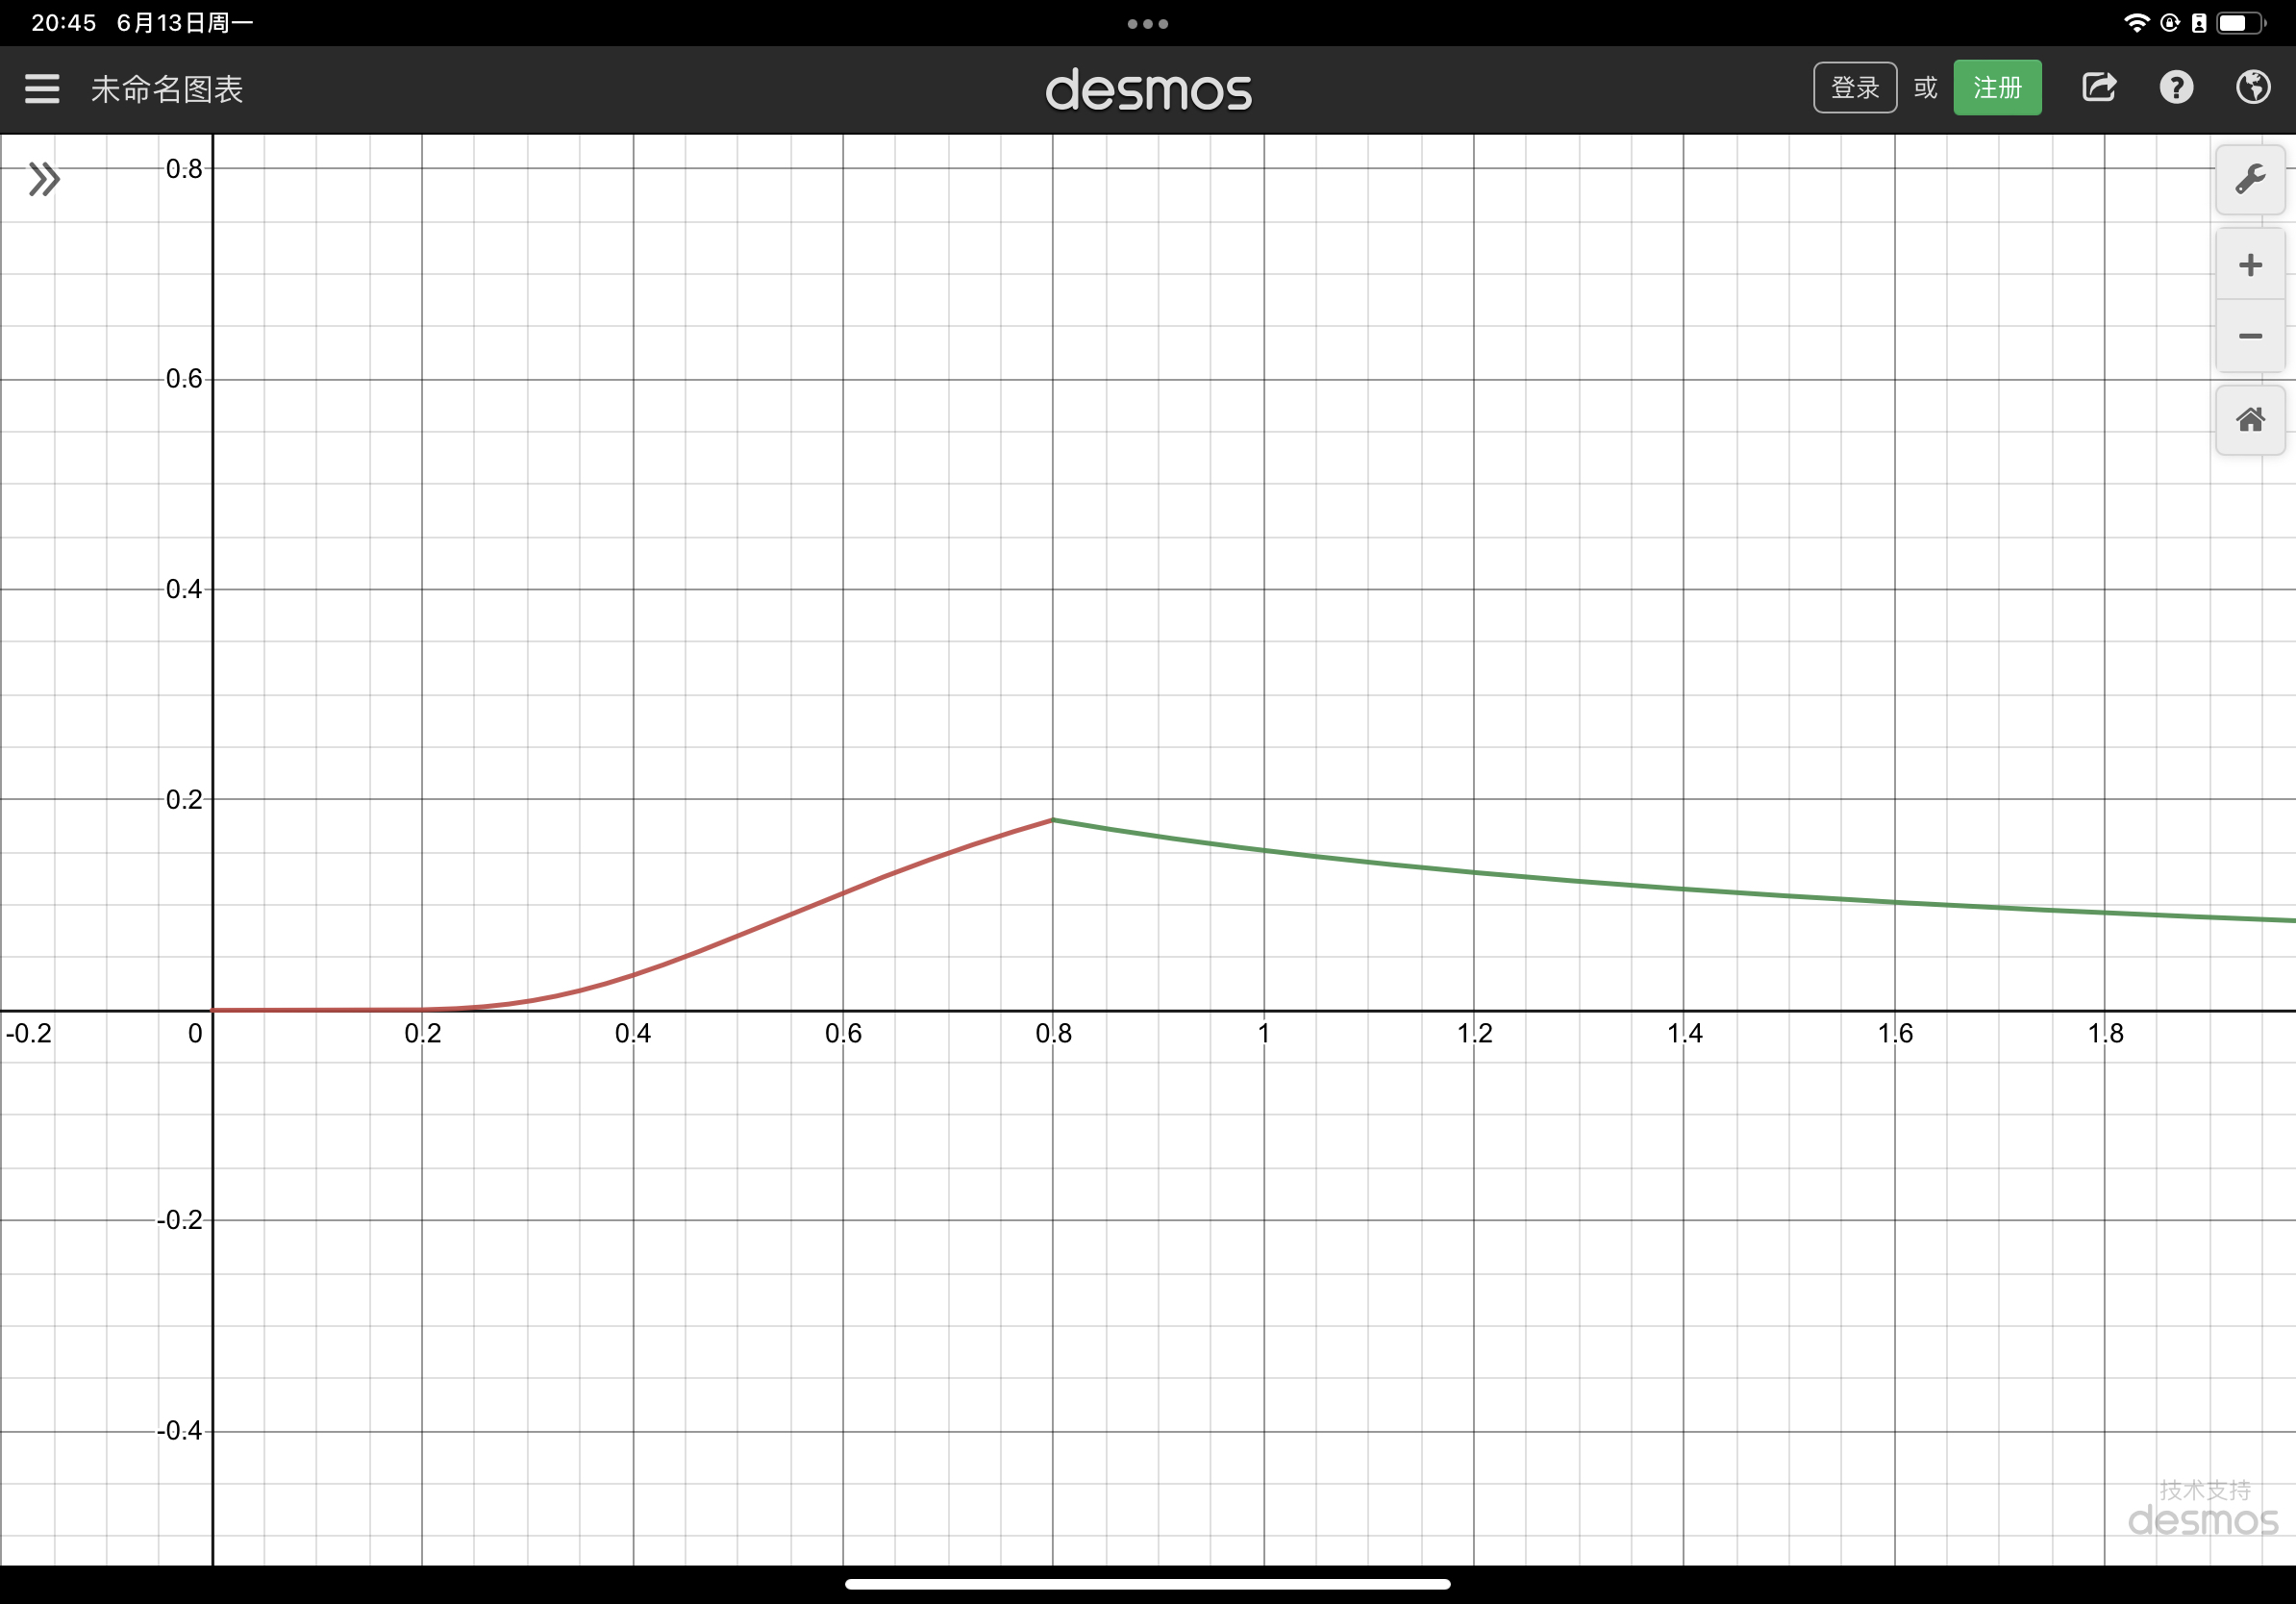
\includegraphics[width = 120mm]{22.5.jpeg}
	\caption{\text{反铁磁体系磁化率随温度变化曲线}}
\end{figure}



\end{enumerate}
\end{tcolorbox}


\end{enumerate}

\end{document}